\lecture{PRACTICAL: SQL Summary}{2023-03-30}{14:00}{Mark}{FTC 3}

T1. Connect to \verb|lib22| database\\
\begin{sql}
\c lib22
\end{sql}

T2. Run the following code to enter a new row of data then run through the tutor tasks above
\begin{sql}
INSERT INTO LIBUSER VALUES ('AAA87857654', 'Lesya', NULL, 'Harrison', 'bharrison66@gov.uk', '1 The Avenue', 'Fratton', 'PO99 5GG');
\end{sql}

\begin{pseudo}
lib22=# Select count(fname) from libuser;
 count
-------
    26
(1 row)

lib22=# select fname, count(fname) from libuser GROUP BY fname;
   fname   | count
-----------+-------
 Arron     |     1
 Millard   |     1
 Sheelagh  |     1
 Ethel     |     1
 Drake     |     1
 Julieta   |     1
 Anastasia |     1
 Quincey   |     1
 Lesya     |     2
 Gibb      |     1
 Madelina  |     1
 Rossy     |     1
 Stewart   |     1
 Zorine    |     1
 Elana     |     1
 Cassie    |     1
 Baryram   |     1
 Gordon    |     1
 Emmeline  |     1
 Konstanze |     1
 Rodolfo   |     1
 Marshall  |     1
 Fernanda  |     1
 Germain   |     1
 Olympia   |     1
(25 rows)

lib22=# select fname, count(fname) from libuser group by fname order by fname;
   fname   | count
-----------+-------
 Anastasia |     1
 Arron     |     1
 Baryram   |     1
 Cassie    |     1
 Drake     |     1
 Elana     |     1
 Emmeline  |     1
 Ethel     |     1
 Fernanda  |     1
 Germain   |     1
 Gibb      |     1
 Gordon    |     1
 Julieta   |     1
 Konstanze |     1
 Lesya     |     2
 Madelina  |     1
 Marshall  |     1
 Millard   |     1
 Olympia   |     1
 Quincey   |     1
 Rodolfo   |     1
 Rossy     |     1
 Sheelagh  |     1
 Stewart   |     1
 Zorine    |     1
(25 rows)

lib22=# select fname, count(fname) as number_of_names from libuser group by fname order by count(fname) desc;
   fname   | number_of_names
-----------+-----------------
 Lesya     |               2
 Millard   |               1
 Sheelagh  |               1
 Ethel     |               1
 Drake     |               1
 Julieta   |               1
 Anastasia |               1
 Quincey   |               1
 Gibb      |               1
 Madelina  |               1
 Rossy     |               1
 Stewart   |               1
 Zorine    |               1
 Elana     |               1
 Cassie    |               1
 Baryram   |               1
 Gordon    |               1
 Emmeline  |               1
 Konstanze |               1
 Rodolfo   |               1
 Marshall  |               1
 Fernanda  |               1
 Germain   |               1
 Arron     |               1
 Olympia   |               1
(25 rows)

lib22=# select fname, count(fname) from libuser group by fname where fname = 'Lesya';
ERROR:  syntax error at or near "where"
LINE 1: ...t fname, count(fname) from libuser group by fname where fnam...
                                                             ^
lib22=# select fname, count(fname) from libuser group by fname having fname = 'Lesya';
 fname | count
-------+-------
 Lesya |     2
(1 row)

lib22=# select fname,mname, lname, count(fname) from libuser group by fname, mname,lname having fname = 'Lesya';
 fname | mname  |    lname    | count
-------+--------+-------------+-------
 Lesya |        | Harrison    |     1
 Lesya | Bidget | Shackleford |     1
(2 rows)
\end{pseudo}

T3. Draw an ERD, (entity with primary and foreign keys only, attributes NOT needed), to cover the following business rules
\begin{itemize}
    \item A car can be owned by 1 person
    \item 1 person may own 1 or more cars
    \item A car may have many services
    \item Each service is for a single car
\end{itemize}

\begin{figure}[H]
    \centering
    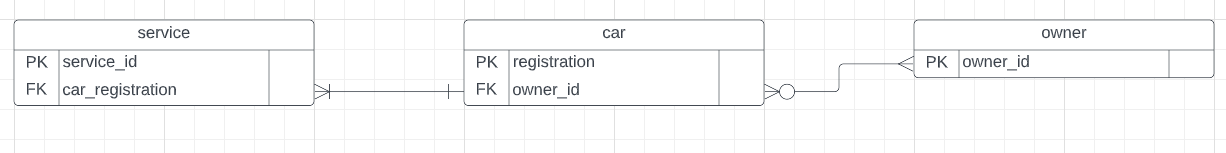
\includegraphics[width=0.9\textwidth]{assets/misc-erd.png}
\end{figure}

T4. Using \verb|lib22|, how many loans have been made by the library?
\begin{sql}
SELECT COUNT(*) FROM LOAN;
\end{sql}
\begin{pseudo}
 count
-------
    30
(1 row)
\end{pseudo}

T5. How many individual books have been lent out? (Think about the individual ISBNs in the loan table).
\begin{sql}
SELECT COUNT(DISTINCT isbn)FROM loan;
\end{sql}
\begin{pseudo}
 count
-------
    12
(1 row)
\end{pseudo}

T6. What is the latest date that we have data for in the loan table?
\begin{sql}
SELECT loanstart FROM loan ORDER BY loanstart DESC LIMIT 1;
\end{sql}
\begin{pseudo}
 loanstart
------------
 2022-11-27
(1 row)
\end{pseudo}

T7. How many books were loaned on the date from Q.6?
\begin{sql}
SELECT COUNT(isbn) FROM loan
WHERE loanstart = '2022-11-27';
\end{sql}
\begin{pseudo}
 count
-------
     1
(1 row)
\end{pseudo}

T8. List the book titles that were loaned between 4th October 2022 and 10th October 2022 (inclusive).
\begin{sql}
SELECT title FROM book
JOIN loan ON book.isbn = loan.isbn
where loanstart BETWEEN '2022-10-04' AND '2022-10-10';
\end{sql}

\begin{pseudo}
                title
-------------------------------------
 FULLY-CONFIGURABLE OPTIMAL FUNCTION
(1 row)
\end{pseudo}

T9. How many books were loaned out between the dates in Q.8? Write a query, don't just count how many results you see.
\begin{sql}
SELECT COUNT(isbn) FROM loan
where loanstart BETWEEN '2022-10-04' AND '2022-10-10';
\end{sql}
\begin{pseudo}
 count
-------
     1
(1 row)
\end{pseudo}

T10. Who wrote the book \verb|De-Engineered Zero Tolerance Graphic Interface|?
\begin{sql}
SELECT CONCAT_WS(' ', authorfname, authorlname) FROM author
JOIN wrote ON author.authorid = wrote.authorid
JOIN book on wroteisbn = isbn
WHERE UPPER(title) = UPPER('De-Engineered Zero Tolerance Graphic Interface');
\end{sql}
\begin{pseudo}
   concat_ws
----------------
 Corbie Varga
 Sara Hurll
 Linet Aberhart
(3 rows)
\end{pseudo}

T11. How many times has the book in Q.10 been loaned out of the library?
\begin{sql}
SELECT count(loan.isbn) FROM loan
JOIN book ON book.isbn = loan.isbn
WHERE UPPER(book.title) = UPPER('De-Engineered Zero Tolerance Graphic Interface');
\end{sql}
\begin{pseudo}
 count
-------
     0
(1 row)
\end{pseudo}

T12. List all users who have NOT loaned books out of the library. (It is up to you what data you need to display)
\begin{sql}
SELECT fname, lname FROM libuser
FULL OUTER JOIN loan ON loan.loanlibrarynumb = libuser.librarynumber
WHERE loanlibrarynumb IS NULL;
\end{sql}
\begin{pseudo}
   fname   |   lname
-----------+-----------
 Germain   | Remmers
 Konstanze | Tonge
 Gibb      | Burgin
 Arron     | Loukes
 Drake     | New
 Cassie    | Dowgill
 Quincey   | Hazle
 Marshall  | Yeudall
 Stewart   | Skill
 Zorine    | Sucre
 Elana     | Matthewes
 Julieta   | Hardison
 Lesya     | Harrison
 Gordon    | Farady
 Madelina  | Sinkins
 Sheelagh  | Ganforthe
 Rodolfo   | Pinks
(17 rows)
\end{pseudo}


T13. Which keyword forces an attribute to only have one version of a value in a table?
\begin{sql}
UNIQUE
\end{sql}

T14. Change the following code to enforce the behaviour in Q.13 on the email attribute.
\begin{sql}
create table test_table (
    test_id int primary key, 
    fname varchar(30) not null, 
    name varchar(30), 
    lname varchar(50) not null, 
    email varchar(70) UNIQUE not null
);
\end{sql}

T15. Using the following attribute names, constraints and datatypes, create a table that connects to the table in Q.14. Call this table \verb|test_table2|
\begin{itemize}
    \item \verb|test_id2| - int primary key
    \item \verb|linking_att| - int foreign key
    \item \verb|notes| - text
\end{itemize}
\begin{sql}
CREATE TABLE test_table2(
    test_id2 INT PRIMARY KEY,
    linking_att INT REFERENCES test_table(test_id),
    notes text
);
\end{sql}

